% !TeX program = xelatex
% ↑ Automatische Auswahl für XeLaTeX compiler

% Das ist mein Template für die TX000 Arbeiten. Nicht perfekt, also falls ihr Verbesserungsvorschläge habt, stellt gerne einen Pull-Request. https://github.com/NikomitK/TX000_Template
% Bitte lasst auch einen star auf github da, danke.
% Wenn ihr die cite funktion von LaTeX nutzen wollt, müsst ihr einfach die Quellen im bibtex Format in die sources.bib datei kopieren, google scholar z.B. hat bei den Quellen einen Button mit dem man das so bekommt, auch viele andere websites.
% Bilder kommen in den images Ordner, den müsst ihr beim abrufen eines Bildes nicht angeben, passiert automatisch.


% Trag hier deine Daten ein, die entsprechenden Felder werden automatisch angepasst.
\def\meinTitel{Das Rucksackproblem}
\def\artDerArbeit{HAUSARBEIT}
\def\meinName{Alexander Regemann, Sven Sendke}
\def\meinKurs{TINF22F}
\def\meineMatrikelNr{4296627 \& 8469950}
\def\modul{Diskrete Mathematik}
\def\abteilungsName{Abteilungsname}
\def\projektBetreuer{Vorname Nachname}
\def\dozent{Dipl.-Math. Christian Kratochwil}
\def\abgabeDatum{15.07.2024}
%-----------------------------------------------------------------------------------


\documentclass[12pt]{report}
\usepackage[heightrounded]{geometry}
\geometry{
	a4paper,
	lmargin=2.5cm, %Seitenrand left
	tmargin=2.5cm, %Seitenrad top
	headsep=35pt %Abstand von Kopfzeile
}
\usepackage[onehalfspacing]{setspace}
\usepackage[compact]{titlesec}
\usepackage{cite} % Zitierungen
\usepackage{struktex} % Struktogramme
\usepackage{array} % kp hat chatgpt benutzt
\usepackage{longtable} % Tabelle über einen seitenumbruch
\usepackage[nohyperlinks, printonlyused]{acronym} % abkürzungsverzeichnis
\usepackage{fontspec}
\usepackage{blindtext} %LoremIpsum
\usepackage{fancyhdr} %Kopf- und Fußzeile
\usepackage[export]{adjustbox} %Bilder alignment
\usepackage{stfloats} %Tabular at bottom
\usepackage{amsmath}
\usepackage{algorithm}
\usepackage{algpseudocode}

\usepackage{blindtext}

\usepackage[utf8]{inputenc} % this is needed for umlauts
\usepackage[ngerman]{babel} % this is needed for umlauts
\usepackage[T1]{fontenc}    % this is needed for correct output of umlauts in pdf


\usepackage{subcaption} % Für subfigures glaub


\usepackage{tikz} % Zum zeichnen
\usetikzlibrary{calc}
\usetikzlibrary{shapes.geometric, arrows}
\setmainfont{Arial}

%--------------------Flowcharts--------------------
\tikzstyle{startstop} = [rectangle, rounded corners, minimum width=3cm, minimum height=1cm,text centered, draw=black, fill=red!30]
\tikzstyle{io} = [trapezium, trapezium left angle=70, trapezium right angle=110, minimum width=3cm, minimum height=1cm, text centered, draw=black, fill=blue!30]
\tikzstyle{process} = [rectangle, minimum width=3cm, minimum height=1cm, text centered, draw=black, fill=orange!30]
\tikzstyle{decision} = [diamond, minimum width=3cm, minimum height=1cm, text centered, draw=black, fill=green!30]
\tikzstyle{arrow} = [thick,->,>=stealth]
%--------------------------------------------------


%--------------------Codeblöcke--------------------
\usepackage{listings} %Für Codeblöcke
\usepackage{color} %Farben für Codeblöcke?
\definecolor{dkgreen}{rgb}{0,0.6,0}
\definecolor{gray}{rgb}{0.5,0.5,0.5}
\definecolor{mauve}{rgb}{0.58,0,0.82}

\lstset{
	language=Java,
	aboveskip=3mm,
	belowskip=3mm,
	showstringspaces=false,
	columns=flexible,
	basicstyle={\small\ttfamily},
	numbers=none,
	numberstyle=\tiny\color{gray},
	keywordstyle=\color{blue},
	commentstyle=\color{dkgreen},
	stringstyle=\color{mauve},
	breaklines=true,
	breakatwhitespace=true,
	tabsize=3
}
%-------------------------------------------------

\usepackage{graphicx} %Package für Bilder
\graphicspath{ {./images/} } %Ordner für Bilder

\sloppy % damit lange Wörter nicht über die Zeile hinausgeschrieben werden.

%--------------------Chapter Heading--------------------
\makeatletter
\def\@makechapterhead#1{%
	\vspace*{-20\p@}%
	{\parindent \z@ \raggedright \normalfont
		\ifnum \c@secnumdepth >\m@ne
		%\huge\bfseries \@chapapp\space \thechapter
		\Huge\bfseries \thechapter.\space%
		%\par\nobreak
		%\vskip 20\p@
		\fi
		\interlinepenalty\@M
		\Huge \bfseries #1\par\nobreak
		\vskip 20\p@
}}
\makeatother
\makeatletter
\def\@makeschapterhead#1{%
	\vspace*{-20\p@}%
	{\parindent \z@ \raggedright \normalfont
		%\huge\bfseries \@chapapp\space \thechapter
		\Huge\bfseries\space%
		%\par\nobreak
		%\vskip 20\p@
		\interlinepenalty\@M
		\Huge \bfseries #1\par\nobreak
		\vskip 20\p@
}}
\makeatother
%-------------------------------------------------------

%\addto\captionsngerman{\renewcommand{\listfigurename}{}}
 % titel von abbildungsverzeichnis weg?

\setlength\parindent{0pt} %Auto Einrücken deaktivieren


%-------------Setup für Inhaltsverzeichnis--------------
\renewcommand{\contentsname}{Inhaltsverzeichnis} %Umbenennung TOC

\usepackage{tocloft} % Formatierung TOX

\setlength{\cftbeforetoctitleskip}{0pt}

\renewcommand{\cfttoctitlefont}{\huge\bfseries}
\renewcommand{\cftloftitlefont}{\huge\bfseries}

\renewcommand\cftchapfont{\Large\bfseries}
\renewcommand\cftchappagefont{\large}

\renewcommand\cftsecfont{\large\bfseries}
\renewcommand\cftsecpagefont{\large}

\renewcommand\cftsubsecfont{\large}
\renewcommand\cftsubsecpagefont{\large}

\renewcommand\cftsubsubsecfont{\normalsize}
\renewcommand\cftsubsubsecpagefont{\normalsize}


\renewcommand\cftchapafterpnum{\par\addvspace{8pt}}
\renewcommand\cftsecafterpnum{\par\addvspace{8pt}}
\renewcommand\cftsubsecafterpnum{\par\addvspace{6pt}}
\renewcommand\cftsubsubsecafterpnum{\par\addvspace{6pt}}
%-------------------------------------------------------


%------------------Setup für LoF/LoT--------------------
\makeatletter
\renewcommand{\@cftmakeloftitle}{}
\renewcommand{\@cftmakelottitle}{}
\makeatother
\setlength{\cftfigindent}{0em} % change indentation of e.g. "Figure 1" within list of figures
\renewcommand\cftfigfont{\large}
\renewcommand\cftfigpagefont{\large}
\setlength{\cfttabindent}{0em} % change indentation of e.g. "Figure 1" within list of figures
\renewcommand\cfttabfont{\large}
\renewcommand\cfttabpagefont{\large}
\setlength{\cftbeforeloftitleskip}{0pt}
\setlength{\cftbeforelottitleskip}{0pt}
%-------------------------------------------------------


%----------------Setup für Verlinkungen-----------------
\usepackage{hyperref}
\hypersetup{
	colorlinks,
	citecolor=black,
	filecolor=black,
	linkcolor=black,
	urlcolor=black
}
%-------------------------------------------------------


%-------------Kopf-/Fußzeile für Titlepage--------------
\fancypagestyle{titlepage}
{
	\fancyhead[L]{
\includegraphics[scale=0.09]{firmenlogo}}
	\fancyhead[R]{
\includegraphics[scale=0.25]{dhbw}}
	\renewcommand{\headrulewidth}{0pt}
	\fancyfoot[C]{}
}
%-------------------------------------------------------

\begin{document} 
	\begin{titlepage}
		\thispagestyle{titlepage}
		\newcommand\HRule{\rule{\textwidth}{1pt}} %Titellinien

		
		\begin{center}
			
			\vspace*{2cm}
			
			%Title
			\begin{spacing}{2}
				{ \huge \bfseries \MakeUppercase{\meinTitel}}
				%{ \large \bfseries subTitle}\\[0.4cm]
			\end{spacing}
			
			\vspace*{1.5cm}
			
			%Art der Arbeit
			\Large \artDerArbeit
			
			\vspace*{3cm}
			
			%Hochschule
			{\LARGE Studiengang Informatik}\\
			{\LARGE an der Dualen Hochschule}\\
			{\LARGE Baden-Württemberg Stuttgart}\\

			\vspace*{2.5cm}
			
			\Large von \meinName
			
			\vspace*{1.5cm}
			
			\Large Abgabedatum: \abgabeDatum

			\begin{table*}[bp]
				\begin{tabular}{l l l l}
					Kurs: & \meinKurs & Matrikelnummer: & \meineMatrikelNr  \\
					Modul: & \modul & Dozent: & \dozent\\
				\end{tabular}
			\end{table*}
			
			
		\end{center}
		
	\end{titlepage}


%------------------Kopf- und Fußzeile-------------------
%\spacing{1.5}

\fancypagestyle{plain}{
	\fancyfoot[L]{\meinName\\
		 \meinKurs}
	\fancyfoot[C]{Seite \thepage\ }% von \pageref{LastPage}}
	\fancyfoot[R]{\abgabeDatum}
}

\pagestyle{plain}
\fancyhead{}


\fancyhead[L]{
\includegraphics[scale=0.09]{firmenlogo}}
\fancyhead[C]{\nouppercase\leftmark}
\fancyhead[R]{
\includegraphics[scale=0.25]{dhbw}}

\renewcommand{\footrulewidth}{0.4pt} %Linie für Fußzeile


\renewcommand{\sectionmark}[1]{\markboth{#1}{}} 
%-------------------------------------------------------

\pagenumbering{Roman}
\newpage
\chapter*{Abstract}
\addcontentsline{toc}{chapter}{\protect\numberline{}Abstract}
Hier kommt der Abstract.
\newpage

%------------------Inhaltsverzeichnis-------------------

\addcontentsline{toc}{chapter}{\protect\numberline{}Inhaltsverzeichnis}
\tableofcontents
\addtocontents{toc}{}
\thispagestyle{plain}
%-------------------------------------------------------
%********************************
%Abbildungsverzeichnis
%********************************
\newpage
\chapter*{Abbildungsverzeichnis}
\addcontentsline{toc}{chapter}{\protect\numberline{}Abbildungsverzeichnis}

\listoffigures




%********************************
%Tabellenverzeichnis
%********************************
\newpage
\chapter*{Tabellenverzeichnis}
\addcontentsline{toc}{chapter}{\protect\numberline{}Tabellenverzeichnis}

\listoftables


\newpage
\chapter*{Abkürzungsverzeichnis}
\addcontentsline{toc}{chapter}{\protect\numberline{}Abkürzungsverzeichnis}
\markboth{Abkürzungsverzeichnis}{Abkürzungsverzeichnis} %Benötigt, damit das im header steht

%********************************
%Abkürzungsverzeichnis
%********************************
\begin{acronym}[SOAP]
	\acro{BA}{Beispiel Acronym}
\end{acronym}


%Speichern des page counters, um bei Literaturverzeichnis weiter zu zählen.
\newcounter{frontmatterPage}
\addtocounter{frontmatterPage}{\value{page}} 

\newpage
\pagenumbering{arabic}
\chapter{Einleitung}
%********************************
%Einleitung
%********************************
Das Rucksackproblem ist eines der bekanntesten und am häufigsten untersuchten Probleme in der Informatik und der mathematischen Optimierung. Es gehört zu den klassischen NP-schweren Problemen und findet in verschiedensten Anwendungsgebieten Anwendung, von der Logistik über die Finanzplanung bis hin zur Produktionsplanung. Die grundlegende Idee des Rucksackproblems besteht darin, eine begrenzte Kapazität eines Rucksacks optimal zu nutzen, um Gegenstände mit unterschiedlichen Werten und Größen auszuwählen. 

%********************************
%Aufgabenstellung
%********************************
\section{Problemstellung}
Das Rucksackproblem birgt trotz seiner scheinbaren Einfachheit eine erhebliche Schwierigkeit, die sich aus seiner exponentiellen Komplexität ergibt. Die Suche nach der optimalen Kombination von Gegenständen, um ie dKapazität des Rucksacks zu maximieren, erfordert eine umfassende Untersuchung aller möglichen Kombinationen. Diese exponentiell wachsende Anzahl von Kombinationen macht das Problem selbst für moderne Computerressourcen schwierig. Effiziente Algorithmen zur Lösung des Problems sind daher von entscheidender Bedeutung.


%********************************
%Vorüberlegung
%********************************
\section{Ziel und Struktur der Hausarbeit}
Ziel dieser Hausarbeit ist es, das Rucksackproblem vorzustellen, mögliche Lösungsansätze zu betrachten und abschließend das Problem anhand eines Beispiels zu untersuchen. 


%********************************
% Grundlagen des Rucksackproblems
%********************************
\newpage
\chapter{Grundlagen des Rucksackproblems}


%********************************
% Definition
%********************************
\section{Definition}
%Das Rucksackproblem ist ein klassisches Optimierungsproblem aus der Kombinatorik. Gegeben ist
%eine Menge von Objekten $U$, wobei jedem Objekt $u \in U$ ein Gewicht $w(u)$ und ein Nutzenwert $v(u)$
%zugeordnet sind. Zusätzlich gibt es eine Gewichtsschranke $B$, die angibt, wie viel Gewicht maximal
%transportiert werden kann.

%Das Ziel des Rucksackproblems ist es, eine Teilmenge $K \subseteq U$ zu finden, die das Gesamtgewicht
%$$\sum_{u \in K} w(u) \leq B$$
%nicht größer als $B$ macht und gleichzeitig den Gesamtnutzen
%$$\sum_{u \in K} v(u)$$
%maximiert.


Das Rucksackproblem ist ein klassisches Optimierungsproblem der Informatik und der Mathematik aus dem Bereich der Kombinatorik, bei dem es um die Frage geht, wie eine begrenzte Menge von Gegenständen, die jeweils ein bestimmtes Gewicht und einen bestimmten Wert haben, so in einen Rucksack mit begrenzter Tragfähigkeit gepackt werden kann, dass der Gesamtwert der darin enthaltenen Gegenstände maximiert wird. Zur Veranschaulichung des Problems dient die grafische Darstellung des Rucksackproblems (siehe Abbildung \ref{fig:rucksackproblem}). 

\begin{figure}[h]
	\centering
	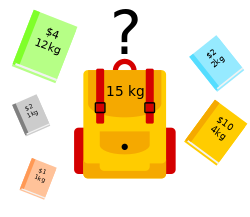
\includegraphics[width=0.5 \linewidth]{Knapsack_Problem_Illustration}
	\caption{Rucksackproblem anhand eines Beispiels}
	\label{fig:rucksackproblem}
\end{figure}

Das Problem ist NP-vollständig und kann mathematisch wie folgt formuliert werden:

Gegeben sei eine Menge $U$ von Objekten. Jedem Objekt $u \in U$ wird ein Gewicht $w(u)$ und ein Nutzenwert $v(u)$ zugeordnet. Es gibt außerdem eine Gewichtsschranke $B \in \mathbb{R}$.

Gesucht ist eine Teilmenge $K \subseteq U$, die die Bedingung

$$\sum_{u \in K} w(u) \leq B$$

einhält und die Zielfunktion

$$\sum_{u \in K} v(u)$$

maximiert. \cite{kellerer2004knapsack}



%********************************
% Anwendungsgebiete
%********************************
\section{Anwendungsgebiete}
Das Rucksackproblem findet in vielen Bereichen der realen Welt Anwendung. Hier einige Beispiele:

\begin{itemize}
	\item \textbf{Ressourcenoptimierung:}
	\begin{itemize}
		\item \textbf{Zuschnitt von Rohmaterialien:} Das Rucksackproblem kann verwendet werden, um den Verschnitt beim Zuschnitt von Rohmaterialien zu minimieren.\cite{kellerer2004knapsack} 
		\item \textbf{Auswahl von Investitionen:} Das Rucksackproblem kann verwendet werden, um die optimale Auswahl von Investitionen für ein Portfolio zu finden.\cite{kellerer2004knapsack}
		\item \textbf{Auswahl von Vermögenswerten:} Das Rucksackproblem kann verwendet werden, um die optimale Auswahl von Vermögenswerten für eine Asset-Backed Securitization zu finden.\cite{kellerer2004knapsack}
	\end{itemize}
	\item \textbf{Kryptographie:}
	\begin{itemize}
		\item \textbf{Generierung von Schlüsseln:} Das Rucksackproblem kann verwendet werden, um Schlüssel für kryptographische Systeme wie das Merkle-Hellman-Kryptosystem zu generieren.\cite{kellerer2004knapsack}
	\end{itemize}
\end{itemize}

%********************************
% Komplexitätsanalyse
%********************************
\section{Komplexitätsanalyse}
%\cite{martello1987algorithms}
%The decision problem form of the knapsack problem (Can a value of at least V be achieved without exceeding the weight W?) is NP-complete, thus there is no known algorithm that is both correct and fast (polynomial-time) in all cases.
%https://en.wikipedia.org/wiki/Knapsack_problem#cite_note-3
Das Rucksackproblem gehört zur Komplexitätsklasse NP (nichtdeterministisch polynomielle Zeit). Dies bedeutet, dass das Problem mit einem deterministischen Algorithmus nicht in Polynomialzeit gelöst werden kann, sofern P ≠ NP. Eine Lösung in pseudopolynomieller Zeit kann jedoch z.B. mit Hilfe der dynamischen Programmierung gefunden werden. \cite{assi8672677}
Im Folgenden sollen nun drei Lösungsmöglichkeiten betrachtet werden.


%********************************
% Dynamisches Programmieren
%********************************
\newpage
\chapter{Dynamisches Programmieren}
Im ersten Schritt wird der Ansatz der dynamischen Programmierung betrachtet.
%********************************
% Prinzip des dynamischen Programmierens
%********************************
\section{Prinzip des dynamischen Programmierens}
Dynamisches Programmieren basiert auf der Idee, ein Problem in kleinere Teilprobleme zu zerlegen und deren Lösungen zu speichern, um sie später wiederzuverwenden. Indem wir die Teilproblemlösungen systematisch kombinieren, können wir das Gesamtproblem effizient lösen. Dieser Ansatz ist besonders nützlich bei Problemen mit überlappenden Teilstrukturen, bei denen viele Teilprobleme mehrmals auftreten. Das dynamische Programmieren ermöglicht eine optimale Lösung, indem es die Gesamtoptimalität aus lokalen optimalen Lösungen aufbaut.\cite{cormen2022introduction}
% \cite{pferschy1999dynamic}

%********************************
%Iwas eigenes
%********************************
\section{Implementierung des dynamischen Programmierens für das Rucksackproblem}
\begin{algorithm}
	\caption{Dynamisches Programmieren für das Rucksackproblem}
	\begin{algorithmic}[1]
		\State \textbf{Input:} Liste von Gegenständen mit Gewicht $w_i$ und Wert $v_i$, maximales Gewicht $W$ des Rucksacks
		\State \textbf{Output:} Maximale Wertsumme, die in den Rucksack passt
		
		\State Initialisiere ein 2D-Array $dp$ mit Dimensionen $(n+1) \times (W+1)$ mit allen Einträgen auf $0$, wobei $n$ die Anzahl der Gegenstände ist
		
		\For{$i \gets 1$ to $n$}
		\For{$j \gets 0$ to $W$}
		\If{$w_i \leq j$}
		\State $dp[i][j] \gets \max(dp[i-1][j], dp[i-1][j-w_i] + v_i)$
		\Else
		\State $dp[i][j] \gets dp[i-1][j]$
		\EndIf
		\EndFor
		\EndFor
		
		\State \textbf{return} $dp[n][W]$
	\end{algorithmic}
\end{algorithm}


%********************************
%Iwas eigenes
%********************************
%\section{Laufzeitanalyse und Komplexität}

%********************************
%Lösung
%********************************
\chapter{Greedy-Algorithmen}

%The idea of the greedy algorithm for the problem (1) consists in a consecutive selection of items with the largest weight density cj=aj as long as the
%knapsack capacity admits it. More formally, the algorithm starts with a feasible solution x ¼ ð0; ... ; 0Þ and consecutively replaces zeros by ones in the
%order of decreasing ratios cj=aj (i.e., from the left to the right); each time the
%feasibility of the corresponding solution is checked. The process terminates
%after obtaining the last feasible solution. This solution xG is called the greedy
%solution; the corresponding objective function value is denoted by f G
%\cite{diubin2003average}


%********************************
%Iwas eigenes
%********************************
\section{Prinzip der Greedy-Algorithmen}
Die Idee des Greedy-Algorithmus für das Rucksackproblem besteht darin, Elemente fortlaufend nach ihrer Gewichtsdichte \( c_j = \frac{a_j}{w_j} \) auszuwählen, solange die Kapazität des Rucksacks dies zulässt. Der Algorithmus beginnt mit einer Anfangslösung \( x = (0, \ldots, 0) \) und ersetzt schrittweise Nullen durch Einsen, und zwar in der Reihenfolge abnehmender Gewichtsdichte \( c_j \) (also von den am besten zu den weniger gut geeigneten Elementen). Bei jedem Schritt wird überprüft, ob die neue Lösung noch machbar ist, das heißt, ob die Gesamtgewichte die Kapazität des Rucksacks nicht überschreiten.

Der Prozess endet, sobald keine weiteren Elemente mehr hinzugefügt werden können, ohne die Kapazität zu überschreiten. Die so gefundene Lösung \( x_G \) wird als gierige Lösung bezeichnet. \cite{diubin2003average}

%Die Idee des Greedy Algorithmus für das Problem besteht in einer fortlaufenden Auswahl von Elementen mit der größten Gewichtsdichte cj=aj, solange die
%Rucksackkapazität dies zulässt. Formal gesehen beginnt der Algorithmus mit einer machbaren Lösung x ¼ ð0; ... ; 0Þ und ersetzt nacheinander Nullen durch Einsen in der
%Reihenfolge der abnehmenden Verhältnisse cj=aj (d.h. von links nach rechts);  jedes Mal wird die Machbarkeit der entsprechenden Lösung überprüft. Der Prozess wird beendet
%nachdem die letzte machbare Lösung gefunden wurde. Diese Lösung xG wird als gierige
%Lösung bezeichnet; der entsprechende Zielfunktionswert wird mit f G notiert. \cite{diubin2003average}

%********************************
%Iwas eigenes
%********************************
\section{Beispiele für Greedy-Lösungsansätze}
\begin{algorithm}
	\caption{Greedy-Algorithmus für das Rucksackproblem}
	\begin{algorithmic}[1]
		\State \textbf{Input:} Liste von Gegenständen mit Gewicht $w_i$ und Wert $v_i$, maximales Gewicht $W$ des Rucksacks
		\State \textbf{Output:} Liste von ausgewählten Gegenständen für den Rucksack
		
		\State Sortiere die Gegenstände absteigend nach dem Verhältnis $v_i/w_i$
		\State Initialisiere eine leere Liste $S$ für die ausgewählten Gegenstände
		\State Setze das aktuelle Gesamtgewicht $totalWeight$ des Rucksacks auf $0$
		
		\For{each Gegenstand $i$ in der sortierten Liste}
		\If{$totalWeight + w_i \leq W$}
		\State Füge den Gegenstand $i$ zu $S$ hinzu
		\State Erhöhe $totalWeight$ um $w_i$
		\EndIf
		\EndFor
		
		\State \textbf{return} $S$
	\end{algorithmic}
\end{algorithm}

%********************************
%Iwas eigenes
%********************************
%\section{Vergleich mit dynamischem Programmieren}

%********************************
%Lösung
%********************************
\newpage
\chapter{First fit decreasing}
\section{Prinzip des First fit decreasing}
Der heuristische Ansatz 'First Fit Decreasing' (FFD), sortiert die Gegenstände absteigend nach ihrem Gewicht und packt jeden Gegenstand in den ersten Rucksack, in den er passt. Wenn kein passender Rucksack gefunden wird, wird ein neuer Rucksack erstellt, und der Gegenstand wird in diesen eingefügt. Der FFD-Algorithmus ist einfach zu implementieren und bietet in der Regel gute, wenn auch nicht optimale, Lösungen für das Rucksackproblem. \cite{martello1987algorithms}

\section{Beispiel für First fit decreasing}
\begin{algorithm}
	\caption{Heuristischer Ansatz (First-Fit-Decreasing) für das Rucksackproblem}
	\begin{algorithmic}[1]
		\State \textbf{Input:} Liste von Gegenständen mit Gewicht $w_i$ und Wert $v_i$, maximales Gewicht $W$ des Rucksacks
		\State \textbf{Output:} Liste von ausgewählten Gegenständen für den Rucksack
		
		\State Sortiere die Gegenstände absteigend nach dem Gewicht $w_i$
		\State Initialisiere eine Liste von Rucksäcken $B$ mit einem leeren Rucksack
		
		\For{each Gegenstand $i$ in der sortierten Liste}
		\State $j \gets 1$
		\While{$j \leq |B|$}
		\If{Gegenstand $i$ passt in Rucksack $B[j]$}
		\State Packe Gegenstand $i$ in Rucksack $B[j]$
		\State \textbf{break}
		\EndIf
		\State $j \gets j + 1$
		\EndWhile
		\If{kein passender Rucksack gefunden}
		\State Erstelle einen neuen Rucksack und packe Gegenstand $i$ hinein
		\State Füge den neuen Rucksack zu $B$ hinzu
		\EndIf
		\EndFor
		
		\State \textbf{return} Alle Gegenstände in den Rucksäcken in $B$
	\end{algorithmic}
\end{algorithm}

%********************************
%Lösung
%********************************
%\newpage
%\chapter{Anwendungsbeispiele und Fallstudien}


%********************************
%Iwas eigenes
%********************************
\pagebreak
\section{Praktisches Beispiel für das Rucksackproblem}
%Angenommen, du hast einen Rucksack mit einer maximalen Tragfähigkeit von 15 kg. Du stehst vor der Wahl, welche Gegenstände du mitnehmen möchtest. Jeder Gegenstand hat ein bestimmtes Gewicht und einen bestimmten Nutzen. Deine Aufgabe ist es, die Gegenstände %auszuwählen, die du mitnehmen solltest, um den Gesamtnutzen zu maximieren, ohne das Gewichtslimit des Rucksacks zu überschreiten.

%Hier ist eine Liste von Gegenständen mit ihren Gewichten (in kg) und Nutzen (zum Beispiel in Euro):

%Gegenstand A: Gewicht = 5 kg, Nutzen = 10 Euro
%Gegenstand B: Gewicht = 8 kg, Nutzen = 14 Euro
%Gegenstand C: Gewicht = 3 kg, Nutzen = 7 Euro
%Gegenstand D: Gewicht = 4 kg, Nutzen = 5 Euro
%Das Ziel ist es, die Gegenstände so auszuwählen, dass der Gesamtnutzen maximiert wird, wobei das Gesamtgewicht den Rucksack nicht über 15 kg hinausgeht.

%Eine mögliche Lösung könnte sein:

%Gegenstand A (5 kg) + Gegenstand C (3 kg) + Gegenstand D (4 kg)
%Das Gesamtgewicht beträgt 5 kg + 3 kg + 4 kg = 12 kg, und der Gesamtnutzen beträgt 10 Euro + 7 Euro + 5 Euro = 22 Euro.

%In diesem Beispiel ist die optimale Auswahl von Gegenständen also A, C und D, da sie den Gesamtnutzen maximiert, ohne das Gewichtslimit des Rucksacks zu überschreiten.

Hier ist ein praktisches Beispiel für das  Rucksackproblem unter Verwendung des Greedy-Algorithmus:

Angenommen, du planst eine Wanderung und hast einen Rucksack mit einer maximalen Tragfähigkeit von 10 kg. Du stehst vor der Wahl, welche Ausrüstung du mitnehmen möchtest, um deine Bedürfnisse während der Wanderung zu erfüllen. Jeder Gegenstand hat ein bestimmtes Gewicht und einen bestimmten Nutzen, der angeben kann, wie wichtig oder nützlich er für deine Wanderung ist.

Hier ist eine Liste von Gegenständen mit ihren Gewichten (in kg) und Nutzen (auf einer Skala von 1 bis 10, wobei 10 am nützlichsten ist):

Wasserflasche: Gewicht = 1 kg, Nutzen = 9
Proviant (Snacks): Gewicht = 2 kg, Nutzen = 8
Schlafsack: Gewicht = 3 kg, Nutzen = 7
Erste-Hilfe-Set: Gewicht = 1 kg, Nutzen = 6
Regenjacke: Gewicht = 1.5 kg, Nutzen = 9
Wanderkarte: Gewicht = 0.5 kg, Nutzen = 5
Das Ziel ist es, die Ausrüstung so auszuwählen, dass der Gesamtnutzen maximiert wird, ohne das Gewichtslimit des Rucksacks zu überschreiten.

Anhand des Greedy-Algorithmus würdest du die Gegenstände nacheinander auswählen, beginnend mit demjenigen, der den höchsten Nutzen pro Kilogramm bietet.

Wasserflasche (1 kg) - Nutzen = 9, verbleibendes Gewicht im Rucksack: 9 kg
Regenjacke (1.5 kg) - Nutzen = 9, verbleibendes Gewicht im Rucksack: 7.5 kg
Proviant (Snacks) (2 kg) - Nutzen = 8, verbleibendes Gewicht im Rucksack: 5.5 kg
Schlafsack (3 kg) - Nutzen = 7, verbleibendes Gewicht im Rucksack: 2.5 kg
Erste-Hilfe-Set (1 kg) - Nutzen = 6, verbleibendes Gewicht im Rucksack: 1.5 kg
Das Gesamtgewicht beträgt 1 kg + 1.5 kg + 2 kg + 3 kg + 1 kg = 8.5 kg, und der Gesamtnutzen beträgt 9 + 9 + 8 + 7 + 6 = 39.

%********************************
%Iwas eigenes
%********************************
%\pagebreak
%\section{Fallstudien zur Anwendung von Rucksackproblemlösungen}


%********************************
%Zusammenfassung und Ausblick
%********************************
\newpage
\chapter{Zusammenfassung und Ausblick}
Das Rucksackproblem ist ein grundlegendes Optimierungsproblem der Informatik und Mathematik mit einem breiten Anwendungsspektrum. Trotz seiner scheinbaren Einfachheit ist das Problem aufgrund seiner exponentiellen Komplexität eine Herausforderung. Es gibt verschiedene Lösungsansätze, z.B. die dynamische Programmierung, der Greedy-Algorithmus oder das First-Fit-Descreasing, das eine Lösung in pseudopolynomialer Zeit liefert, deren Lösung aber nicht immer korrekt ist. Die vorgestellten Ansätze bieten verschiedene Herangehensweisen an das Rucksackproblem, aber es gibt noch Raum für weitere Untersuchungen und Verbesserungen. Die Integration von Techniken des Machine-Learning könnte neue Möglichkeiten eröffnen, das Rucksackproblem zu lösen und gleichzeitig den steigenden Anforderungen in verschiedenen Anwendungsbereichen gerecht zu werden.

%********************************
%Literaturverzeichnis
%********************************
\newpage
\pagenumbering{Roman}
\setcounter{page}{\value{frontmatterPage}} %Bei \pagenumbering wird Seitenzähler zurückgesetzt, hier wird der gespeicherte Wert vom frontmatter weitergeführt
\addtocounter{page}{1}
\addcontentsline{toc}{chapter}{\protect\numberline{}Literaturverzeichnis}

%Quellenverzeichnis
\renewcommand{\refname}{Literaturverzeichnis}
\bibliographystyle{IEEEtran}
\bibliography{./sources}


\end{document}
